\documentclass[12pt]{article}
\usepackage{amsfonts,amsthm,amsmath,amssymb,mathtools}
\usepackage{mathrsfs}
\usepackage{enumitem}
\usepackage{tikz-cd}
\usepackage{geometry}
\usepackage{mlmodern}
\usepackage{graphicx}

\geometry{letterpaper, portrait, margin=1in}

\setcounter{section}{0}

\renewcommand{\thesection}{\S\arabic{section}}
\renewcommand{\thesubsection}{\arabic{section}}
\DeclareMathOperator{\im}{im}
\DeclareMathOperator{\id}{id}

\newtheorem{thm}{Theorem}
\newenvironment{theorem}[1]{
	\renewcommand{\thethm}{#1}
	\begin{thm}
		}{\end{thm}}

\newtheorem{lma}{Lemma}
\newenvironment{lemma}[1]{
	\renewcommand{\thelma}{#1}
	\begin{lma}
		}{\end{lma}}

\theoremstyle{definition}
\newtheorem{ex}{Assignment}
\newenvironment{exercise}[1]{
	\renewcommand{\theex}{#1}
	\begin{ex}
		}{\end{ex}}

\title{MTH 732 Topology - Homework 6}
\author{Connor Mooneyhan}
\date{February 26, 2026}

\begin{document}

\maketitle

\begin{ex}
	The following diagram represents an incomplete $\Delta$-complex structure on the genus 2 surface (2-holed torus).
	Arrows have been correctly placed on the edges $a_i$ and $b_i$, but not on the $c_i$.\\
	\begin{center}
		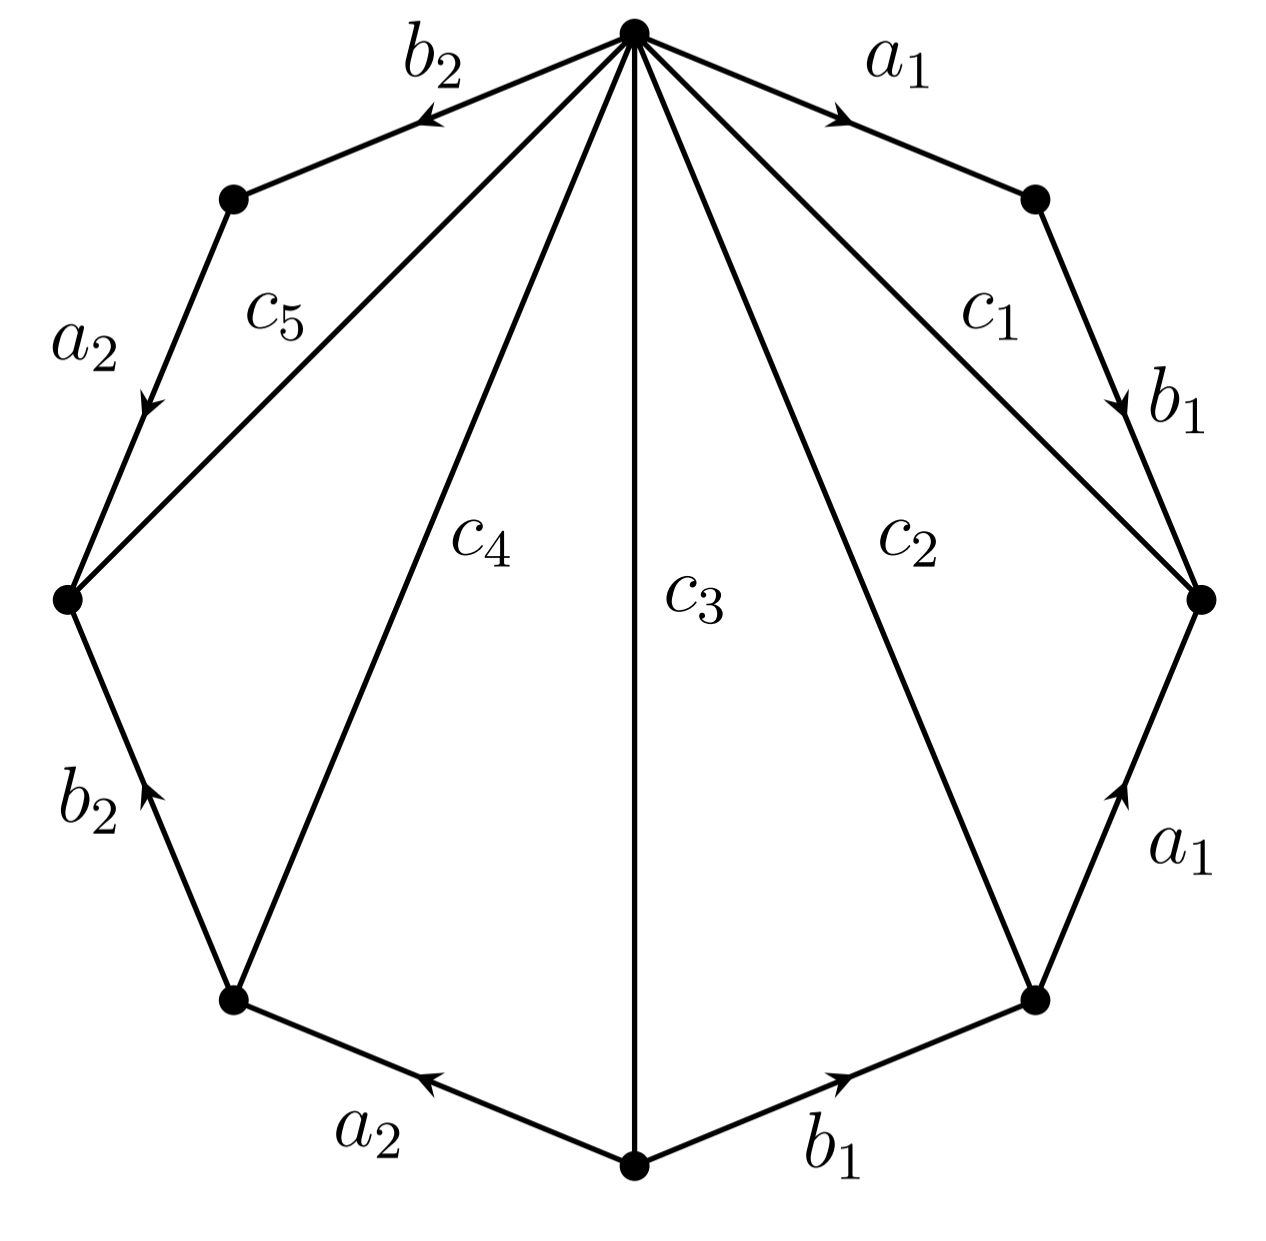
\includegraphics[width=0.4\textwidth]{unlabeled-octagon}\\
	\end{center}
	\begin{enumerate}[label=(\roman*)]
		\item Complete the diagram by orienting the $c_i$ and list all simplices involved (there are 0, 1, and 2-simplices).
		      Keep track of the labels you assign for each simplex.
		\item Compute the boundary maps $\partial_2 : \Delta_2 \to \Delta_1$ and $\partial_1 : \Delta_1 \to \Delta_0$ explicitly.
		      Use the labels from part (i) to say what the map does to each simplex.
		\item Find the homology groups $H_0^\Delta$, $H_1^\Delta$, and $H_2^\Delta$.
		      Check that $H_1^\Delta = \pi_1/[\pi_1, \pi_1]$.
	\end{enumerate}
\end{ex}
\begin{proof}
	\begin{enumerate}[label=(\roman*)]
		\item Our labeling:\begin{center}
			      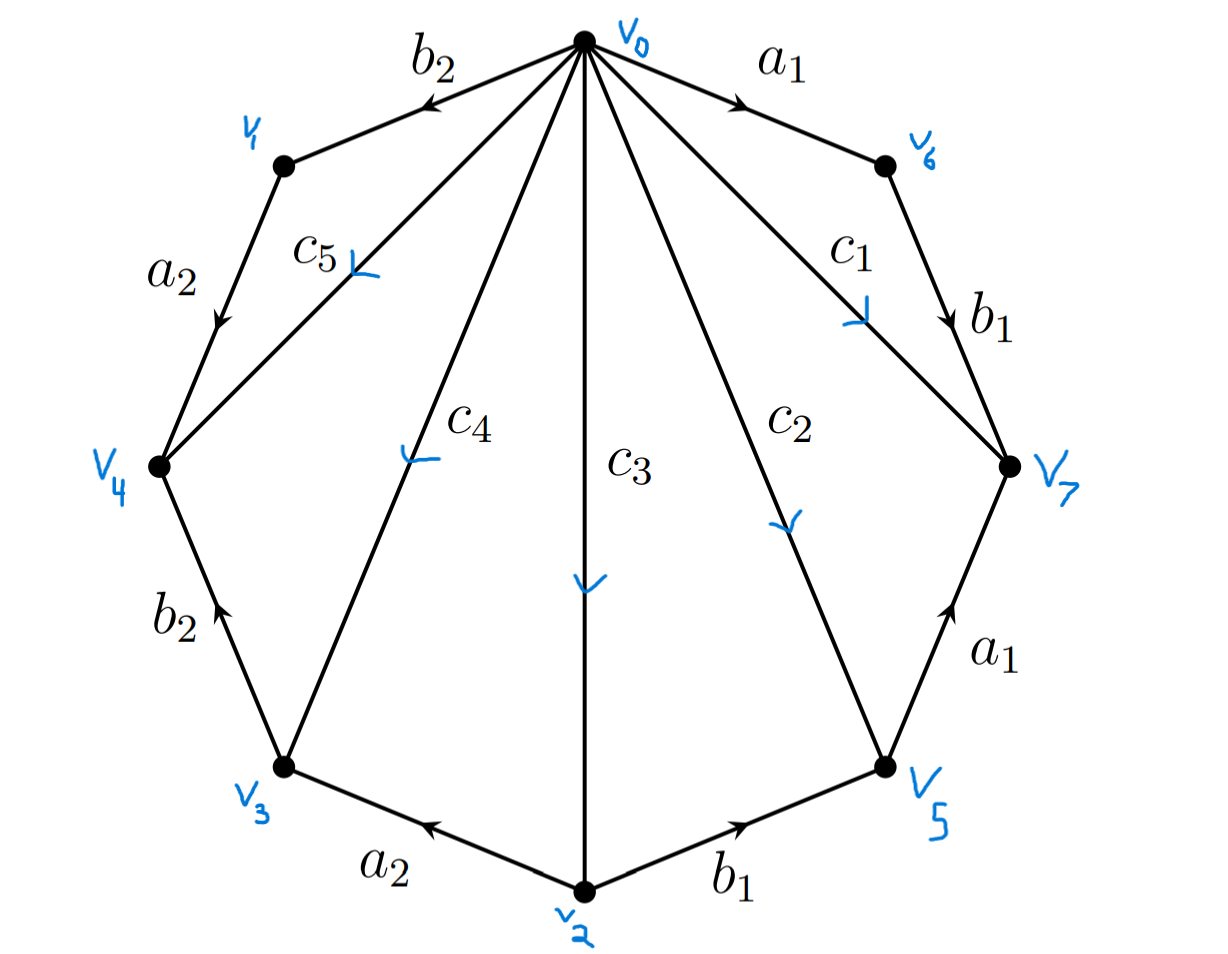
\includegraphics[width=0.7\textwidth]{labeled-octagon}
		      \end{center}
		      Thus the simplices are as follows: \begin{align*}
			      \text{0-simplices} = \lbrace & [v_0], [v_1], [v_2], [v_3], [v_4], [v_5], [v_6], [v_7] \rbrace                                               \\
			      \text{1-simplices} = \lbrace & [v_0, v_1], [v_0, v_4], [v_0, v_3], [v_0, v_2], [v_0, v_5], [v_0, v_7], [v_0, v_6],                          \\
			                                   & [v_1, v_4], [v_3, v_4], [v_2, v_3], [v_2, v_5], [v_5, v_7], [v_6, v_7]\rbrace                                \\
			      \text{2-simplices} = \lbrace & [v_0, v_1, v_4], [v_0, v_3, v_4], [v_0, v_2, v_3], [v_0, v_2, v_5], [v_0, v_5, v_7], [v_0, v_6, v_7] \rbrace
		      \end{align*}
		\item First we compute $\partial_2$: \begin{equation*}
			      \begin{array}{c|c}
				      \sigma \in \Delta_2 & \partial_2(\sigma)                                                                \\
				      \hline
				      [v_0, v_1, v_4]     & [v_1, v_4] - [v_0, v_4] + [v_0, v_1] = a_2 - c_5 + b_2 \\{}
				      [v_0, v_3, v_4]     & [v_3, v_4] - [v_0, v_4] + [v_0, v_3] = b_2 - c_5 + c_4 \\{}
				      [v_0, v_2, v_3]     & [v_2, v_3] - [v_0, v_3] + [v_0, v_2] = a_2 - c_4 + c_3 \\{}
				      [v_0, v_2, v_5]     & [v_2, v_5] - [v_0, v_5] + [v_0, v_2] = b_1 - c_2 + c_3 \\{}
				      [v_0, v_5, v_7]     & [v_5, v_7] - [v_0, v_7] + [v_0, v_5] = a_1 - c_1 + c_2 \\{}
				      [v_0, v_6, v_7]     & [v_6, v_7] - [v_0, v_7] + [v_0, v_6] = b_1 - c_7 + a_1
			      \end{array}
		      \end{equation*}
		      and then $\partial_1$: \begin{equation*}
			      \begin{array}{c|c}
				      \sigma \in \Delta_1 & \partial_1(\sigma)                       \\
				      \hline
				      [v_0, v_1]          & [v_1] - [v_0] \\{}
				      [v_0, v_4]          & [v_4] - [v_0] \\{}
				      [v_0, v_3]          & [v_3] - [v_0] \\{}
				      [v_0, v_2]          & [v_2] - [v_0] \\{}
				      [v_0, v_5]          & [v_5] - [v_0] \\{}
				      [v_0, v_7]          & [v_7] - [v_0] \\{}
				      [v_0, v_6]          & [v_6] - [v_0] \\{}
				      [v_1, v_4]          & [v_4] - [v_1] \\{}
				      [v_3, v_4]          & [v_4] - [v_3] \\{}
				      [v_2, v_3]          & [v_3] - [v_2] \\{}
				      [v_2, v_5]          & [v_5] - [v_2] \\{}
				      [v_5, v_7]          & [v_7] - [v_5] \\{}
				      [v_6, v_7]          & [v_7] - [v_6]
			      \end{array}
		      \end{equation*}
		\item First, since $\partial_0 = \mathbf{0}$, $\ker\partial_0 = \Delta_0$, and since every 1-simplex $[v_i]$ where $i \neq 0$ satisfies $[v_i] - [v_0] \in \im\partial_1$, they all get identified in $H_0^\Delta$, so $H_0^\Delta = \mathbb{Z}$.

		      In $H_1^\Delta$, we have the $c_i$ edges identified as follows: \begin{align*}
			      c_5 & = a_2 + b_2              \\
			      c_4 & = c_5 - b_2 = a_2        \\
			      c_3 & = c_4 - a_2 = 0          \\
			      c_2 & = b_1 + c_3 = b_1        \\
			      c_1 & = a_1 + c_2 = a_1 + b_1,
		      \end{align*}
		      so we can in fact express each $c_i$ in terms of $a_1$, $a_2$, $b_1$, and $b_2$, leaving us with four generators for $H_1^\Delta$.
          Thus $H_1^\Delta \cong \mathbb{Z}^4$.

          Finally, consider that $\Delta_3$ is trivial, so $\im\partial_3$ is trivial, and thus $H_2^\Delta = \ker \partial_2$.
          Since there are 6 generators in $\Delta_2$ and the rank of $\im\partial_2$ is 5 as seen above, $\ker\partial_2$ must have rank 1, and thus $H_2^\Delta \cong \mathbb{Z}$.
	\end{enumerate}
\end{proof}

\begin{ex}
	Show that if $X = \bigsqcup_{i \in I} X_i$ where the $X_i$ are the path components of $X$, then for every $n$, the Abelian groups $C_n(X)$ and $H_n(X)$ split as direct sums: \begin{equation*}
		C_n(X) = \bigoplus_{i \in I} C_n(X_i) \hspace{2em}\text{and}\hspace{2em} H_n(X) = \bigoplus_{i \in I} H_n(X_i).
	\end{equation*}
\end{ex}
\begin{proof}
	Since each singular $n$-simplex is a continuous map, it must map into a single path component $X_i$.
	Thus the free abelian group on all singular $n$-simplices, namely $C_n(X)$, is the direct sum of the free abelian groups on all singular $n$-simplices living in each $X_i$ separately, namely $\bigoplus_{i \in I} C_n(X_i)$.

	Given the above, the kernels of the boundary maps will also split since they are subgroups of the $C_n(X_i)$, and thus we can focus on the images of boundary maps.
	Given a singular $n$-simplex $\sigma$, the boundary $\partial\sigma$ is a $\mathbb{Z}$-linear combination of singular $(n-1)$-simplices, the images of which are subsets of the image of $\sigma$, which we have already noted is a subset of $X_i$.
	A general element of $H_n(X)$ is a coset $A(\im \partial_{n+1})$ where $A \in C_n(X)$ and thus $A = \bigoplus{i=1}^m A_i$ where each $A_i \in C_n(X_i)$, and thus $A(\im\partial_{n+1}) = \sum_{i=1}^m A_i(\im\partial_{n+1})$, so $H_n(X) = \bigoplus_{i \in I} H_n(X_i)$.
\end{proof}

\begin{ex}
	Show that if $X$ is path-connected, $H_0(X) = \mathbb{Z}$.
\end{ex}
\begin{proof}
	For any space $X$, $\ker\partial_0 = C_0(X)$, so $H_0(X) = C_0(X)/\im\partial_1$.
	If $X$ is path-connected, then given any two points $x, y \in X$, $x - y \in \im\partial_1$ since there exists a map from a closed interval (which is itself a singular 1-simplex) to $X$ which starts at $y$ and ends at $x$, and the boundary of that singular 1-simplex (after precomposition with the canonical map from the singular 1-simplex so that it is truly a singular 1-simplex) is $x - y$.
	Thus by definition of the quotient, since $x-y \in \im\partial_1$, $x \sim y$, and thus every point is related to every other point.
	Since $C_0(X)$ is generated by the collection of points in $X$, this collapses the group to one generator.
	We exhibit the map $\varepsilon: C_0(X) \to \mathbb{Z}$ defined by \begin{equation*}
		\varepsilon\left(\sum_{i=1}^m n_i\sigma_i\right) = \sum_{i=1}^m n_i,
	\end{equation*}
	which surjects onto $\mathbb{Z}$, and thus $H_0(X) \cong \mathbb{Z}$.
\end{proof}

\end{document}
